\chapter{Entorno empresarial} \label{entornoEmpresarial}
En este capítulo se describe a la empresa en la cual se desarrolló el proyecto de pasantía. Comprende una breve reseña histórica, su misión y visión, la estructura organizacional y el área a la cual el pasante estuvo asignado.

\section{Antecedentes de la empresa} \label{antecedentesEmpresa}
IKêls Consulting \cite{ikelsAbout}  se creó en el año 2008 en Venezuela como una empresa dedicada al desarrollo de soluciones en el área de Sistemas de Información. Los fundadores contaban con una amplia trayectoria en los procesos y tecnología para la elaboración de documentación técnica avanzada (por ejemplo normas para construcción de plantas petroquímicas).

Para aprovechar la experiencia previa los productos y servicios se concentran en el área de aplicaciones web (por ejemplo, con \ac{CMS}) para el sector corporativo atendiendo a un selecto grupo de clientes con presencia local e internacional.

Actualmente, las actividades principales se concentran en:

\begin{itemize}
  \item Construcción de portales web en múltiples idiomas que pueden ser administrados por sus propios dueños. Esto incluye la programación de módulos especiales para integrar información desde y hacia sistemas externos, desplegar datos de manera amigable o generar notificaciones automáticas dependientes de actividades de los visitantes u otros eventos.
  \item Apoyo en la gestión de contenido de portales web.
  \item Consultoría y gestión para optimizar las variables asociadas al rendimiento y desempeño de las páginas web. Teniendo especial interés en el monitoreo de presencia en buscadores, evaluación del perfil de los visitantes y garantizar un nivel adecuado de usabilidad en diferentes dispositivos, etc.
  \item Desarrollo de productos personalizados que complementen las ventajas y facilidades de los dispositivos móviles en sincronización con mecanismos de soporte en servidores web.
  \item Desarrollo de soluciones especializadas para ofrecer bajo el modelo SaaS o Software as a Service.
\end{itemize}

\section{Misión}
Proveer productos y servicios en el área de sistemas de información que permitan una comunicación efectiva de nuestros clientes con su público y también sirva como plataforma de trabajo donde se aprovechen las innovaciones y ventajas de las tecnologías más modernas \cite{ikelsAbout}.

\section{Visión}
Desean ser proveedores confiables, que ofrecen un alto valor agregado en cada producto o servicio que prestan a sus clientes \cite{ikelsAbout}.

\section{Ubicación del pasante}
El proyecto de pasantía pertenece al grupo de desarrollo de aplicaciones y cuenta con la dirección de la Gerencia General y con el apoyo de los ingenieros líderes del grupo. En la Figura \ref{fig:organigrama} se muestra el organigrama de la empresa.

\begin{figure}[H]
\centering
    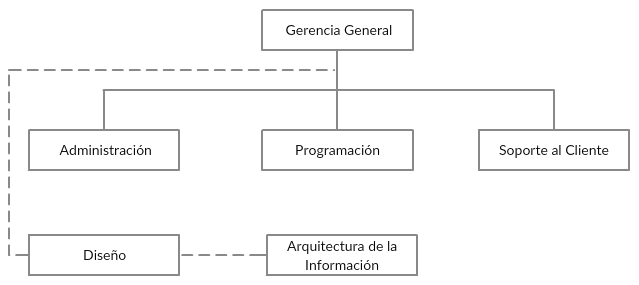
\includegraphics[width=.6\textwidth,height=.6\textheight,keepaspectratio]{organigrama.png}
    \caption{Organigrama de la empresa}
    \label{fig:organigrama}
\end{figure}